%\[B\](.*?)\[/B\] => \\textbf{$1}

\section{Regression}

Regression is used a lot in statistics, where its primary purpose is to predict a target value based on independent predictors and is useful to find cause and effect relationships between variables \cite{linear_regression_ml}. One experiment that might be interesting is to perform linear regression on some of the columns in the demographics dataset \ref{figure:demographics}, in order to see whether there are columns that tell more about the participant's group (control or condition).  

Not all of the columns are relevant though, for example, \textbf{number} is unique for each participant, so it does not make sense to use. The column \textbf{melanch} also does not make sense to use, as there is only one participant with Melancholia. \textbf{Inpatient} cannot be used because the participants in the control group are not patients, and cannot be either inpatient or outpatient. The same goes for \textbf{edu}, \textbf{work} and \textbf{marriage}, but we don't have these data values for control group participants. We don't have their \textbf{afftype} or any of the \textbf{MADRS} scores either, but we already know them: \textbf{afftype} should be 0 (not bipolar) and both \textbf{MADRS} scores should be 0 (not depressed). 

We used the \textbf{afftype} column as a target in the regression. This way we could classify whether a participant is in the control or the condition group, by setting the \textbf{afftype} value to either 0 or 1 instead of 0, 1, 2 or 3 (values above 1 reduced to 1), and ran the regression on all of the remaining columns one by one:

\begin{itemize}
      \item \textbf{Gender}
      \item \textbf{Age}
      \item \textbf{Days}
      \item \textbf{MADRS1}
      \item \textbf{MADRS2}
\end{itemize}

\begin{figure}
  \begin{code}
    \begin{minted}[linenos]{python}
      def regression_model():
        model = Sequential()
        model.add(Dense(5, input_dim=1, activation='relu'))
        model.add(Dense(1))

        model.compile(loss='mse', optimizer='adam', metrics=['mse'])
        return model
    \end{minted}
    \caption{Regression Model}
    \label{code:regression_model}
  \end{code}
\end{figure}

The model for this task is straightforward. We created a sequential model \ref{code:regression_model} with one input layer and one output layer. The input is a \textbf{dense} layer which takes one value (the value of the current column), activates using \textbf{relu} and outputs 5 neurons. In the output layer, we activate using a \textbf{linear} function (default activation function when none are specified) and return one value: the prediction. We compiled the model with the loss function \textbf{Mean Squared Error} and the optimizer \textbf{Adam}. 

Since we were predicting the \textbf{afftype} of a participant, which is a binary value (0 or 1) and a prediction from the model yields a value between 0 and 1, we rounded the prediction value to the nearest integer after running predictions on the test data. Doing it this way instead of making a classification model, makes the \textbf{loss} value more useful as a metric while training rather than accuracy. 

When testing the model, we wanted to achieve an accuracy of 100\% when using the \textbf{MADRS} scores. The task should be easy because of how easy it is using a simple check: if the MADRS score is 0, then the participant is in the control group. If not, the participant is in the condition group. We did not need to use machine learning on these columns but was interesting to train the model to find this relationship without telling it the simple rule. For the other columns, we did not know what to expect; maybe there was a relationship, maybe not.

\section{1D Convolutional Neural Network}

\subsection{Convolution}

\begin{figure}[h]
    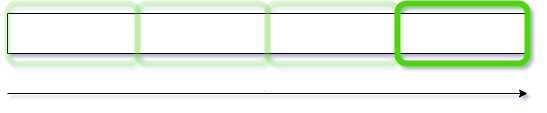
\includegraphics[height=2.5cm]{img/feature_detector.png}
    \caption{Feature Detector / Filter "sliding" over input data}
    \label{figure:feature_detector}
\end{figure}

\noindent The main ingredient in a CNN is the \textit{convolutional} layer. It is responsible for the convolution, which in mathematics is a function derived from two given functions by integration which expresses how the shape of one is modified by the other \cite{convolution_definition}. 

The convolutional layer in machine learning consists of \textit{filters} \ref{figure:feature_detector}, which are the sliding windows that go through the input data.  They are also called \textit{feature detectors}, and using 100 of them means that the layer can detect 100 features. The size of a filter is called \textit{kernel size}. The output of the convolutional layer is a matrix with one column for each filter, and one row for each step in the convolution. How many steps there are, is given by the length of the input data (also called \textit{height}) minus the kernel size plus 1.

\subsection{Creating the Model}
Following the tutorial on 1D Convolutional Neural Networks \cite{1d_cnn}, we came up with two models. One model for the first two goals was built for classification \ref{code:1d_conv_net_classifier}, and for the third goal we came up with another model built for prediction \ref{code:1d_conv_net_predictor}. We built the models a lot like how it was in the tutorial, but we also had to tweak some of the parameters to make the model work on our dataset.

To make a convolutional neural network, you need some \textit{convolutional} and \textit{pooling} layers. Which layers that added in between and the ordering of them, together with the parameters passed to the layers, is what makes the model perform differently. 

\subsubsection{Classification}
The following model \ref{code:1d_conv_net_classifier} is used to achieve our first two goals; classifying whether a participant belongs to the \textbf{control} or \textbf{condition} group, and classifying the participant's \textbf{depression class}. The only difference between these two goals is the number of classes we are trying to classify, and therefore only the output layer needs to be changed.

\begin{enumerate}
      \item We started by defining a \textbf{Sequential} model. This is easy to understand and readable way of defining a model. Alternatively, we could have used a \textbf{functional} model, which would give more control of inputs and outputs of the layers. A \textbf{functional} model would also be useful if we wanted to debug and optimize each layer within the model. 
      
      \item \textbf{Reshape}: In the first layer we needed to reshape the input data so that it becomes an $X$ by 1 matrix, where $X$ is the length of each segment. The reason for the reshape step is because the next layer (\textbf{Conv1D}) requires the input to contain the parameters \textit{batch, steps and channels}. \textit{Batch} will be set to \textbf{None}, \textit{steps} will be the segments, and \textit{channels} will be $1$ (because we only have one measurement value for each minute).
      
      \item \textbf{Conv1D}: This is the first \textit{convolutional} layer, where the required parameters are how many \textit{filters} wanted, and how big the \textit{kernel} should be. As in the tutorial, we also used 100 filters and a kernel size of 10. Having less or more filters might have an impact on the performance, but we did not want to over-complicate the model yet. There are many different parameters that we can use on a layer like this, for example, \textit{padding} and \textit{strides}, but using the default values was a good choice for now. The output of this layer results in a $(X-10+1) \times 100$ matrix, where $X$ is the length of each segment here as well. The activation function for all convolutional layers in this model is \textit{ReLU} (Rectified Linear Unit). 

      \item \textbf{Conv1D}: The second convolutional layer looks exactly like the first one, and the output is a $(X-10+1-10+1) \times 100$ matrix. 
      \item \textbf{MaxPooling1D}: Pooling is important in a convolutional neural network to reduce complexity \cite{1d_cnn}. 
            The basic idea of \textit{max pooling} is to reduce to only the maximum value for each \textit{window} of size $N \times N$. We are using 2 as 
            window size ($N$), resulting in matrix that is half the size of the input: $ \frac{X-10+1-10+1}{2} \times 100$. 
            Pooling may also help reduce \textit{overfitting}, which is when the model learns its training data too well and performs worse on unseen data.
      \item \textbf{Conv1D}: Two more convolutional layers are added, and after these, the input to the next layer will be a matrix of size
            $ \left( \frac{X-10+1-10+1}{2}-10+1-10+1 \right) \times 160 $.
      \item \textbf{GlobalAveragePooling1D}: This is another pooling layer, and this one takes the average of weights within the network instead of the maximum.
            After doing this, the matrix will be of size $ 1 \times 160 $.
      \item \textbf{Dropout}: Dropout is used to reduce overfitting, by randomly ignoring units in the neural network. 
      \item \textbf{Dense}: The final layer in the model is a dense layer (fully connected) which reduces the matrix from $160$ values to 
            either $2$ or $3$ (for goal one and two), with the activation function \textbf{softmax}. 
            Then the output (a $1$ in one of the neurons) is mapped to the corresponding label.
\end{enumerate}

After creating the model, we \textit{compile} it as a model that is ready to be \textit{fit} to the dataset, 
giving it a \textbf{loss function} and an \textbf{optimizer}.The loss function is the function that evaluates how well the 
model \textit{models} the given data \cite{loss_functions}, and the optimizer is the function that attempts to lower the output of the loss function. 

For the first two goals, the loss function \textit{categorical crossentropy} calculates a probability over the 
number of classes that are supplied (number of classes equals the number of neurons in the output layer). 

For the optimizer, there are many different choices available,
but to keep things simple, we will start out using an optimizer called \textbf{Adam} for training all of our models. Using a different optimizer can make the 
model fit to the dataset faster or slower. 

\subsubsection{Prediction}
To make the model work for our third goal, where we will predict the actual value for the participant's MADRS score, we have to change a few layers. To simplify it a bit, we removed two of the \textit{Conv1D} layers and applied this after the \textit{GlobalAveragePooling1D} layer:

\begin{enumerate}
      \setcounter{enumi}{7}
      \item \textbf{Flatten}: The matrix needs to be flat (one dimensional) before proceeding to the final layers.
      \item \textbf{Dense}: A dense layer with $10$ neurons, and \textit{relu} as the activation function. 
      \item \textbf{Dense}: The output layer is a dense layer of size $1$, since we are predicting \textit{one} value. 
            Also, the activation on this layer is going to be \textit{linear} instead of softmax.
\end{enumerate}

We compile this model with the loss function \textit{Mean Squared Error}, which is measured as the average (mean) of squared difference between predictions and actual observations ($ loss = \frac{\sum_{i=1}^{n}(y_i-\hat{y}_i)^2}{n} $) \cite{loss_functions}. The optimizer is the same as before.

\subsection{Creating Input and Output Data}
\begin{table}
  \begin{center}
    \begin{tabular}{| l | l |}
      \hline
      \textbf{Not bipolar} & \textbf{Bipolar}  \\ \hline
      0                    &  1                \\ \hline
      1                    &  0                \\ \hline
      0                    &  1                \\ \hline
      1                    &  0                \\ \hline
      1                    &  0                \\ \hline
      0                    &  1                \\ \hline
      0                    &  1                \\ \hline
      1                    &  0                \\ \hline
    \end{tabular}
    \caption{Categorical Labels}
    \label{table:categorical_labels}
  \end{center}
\end{table}

One function (\textit{create\_segments\_and\_labels()} \ref{code:reading_dataset}) is responsible of creating the data that is sent into the neural network. We start by defining a \textit{segment length} $L$, which is how much data (minutes) we want inside each segment. We will experiment with the value of $L$, but let's say we use segments of 4 hours at a time ($L=4*60=240$). Next, we need a value for how many values to step after each iteration, $S$. We will keep this value at one hour, meaning $S=60$. Between the different goals, this function will only be different in how it determines the output values. The code in the Source Code section \ref{code:reading_dataset} is simplified to only generate input and output for classifying control/condition groups (goal one).

\begin{itemize}
      \item First we read the \textit{global} dataset, where we find each participant and whether they are bipolar or not. As there is no \textit{afftype} value
            for non-bipolar participants, we simply set this to 0. This is fine because the other possible values are 1, 2 and 3.
      \item Then we iterate over all participant activity data files:

      \begin{itemize}
        \item Append a \textbf{segment} that is of length $L$ to the list of segments (using default parameters in the
              \textit{create\_segments\_and\_labels} function \ref{code:reading_dataset}).
        \item Append the target value for the current goal, so:
          \begin{itemize}
                \item Append a $1$ or $0$ for classifying control/condition group.
                \item Append a $0$, $1$ or $2$ for classifying depression class \\(normal/mild/moderate).
                \item Append the MADRS score (after measurement period) when the goal is to predict MADRS score.
          \end{itemize}  
        \item Skip $S$ indexes, and repeat until we have added all segments.
      \end{itemize}

      \item Make the list of labels into a \textit{categorical} 2D matrix \ref{table:categorical_labels} with a \textbf{1} in only one of the columns,
            instead of a single-dimensional list.
            This is only needed in the first two goals, for the \textbf{softmax} activation function.
      \item Also we need the list of segments to be restructured. We do this with the \textbf{reshape} function, 
            and after this, the data is ready to be passed into the neural network.
\end{itemize}

\subsection{Train and test data}
We did one last step before we started training the model. We needed to split the data ion two parts; training and test data. This way we can calculate the performance of the model after training has finished, and also prevent overfitting by evaluating data that is unseen to the model. 

\subsubsection{train\_test\_split}
The function \textit{train\_test\_split} from the \textit{sklearn} package was useful here; we input the segments and labels, plus how large we want the training and test sets to be (number between 0 and 1, which determines the size of the test partition). The function also randomizes the data, preventing model to accidentally learn something correct for segments in a row that also are chronologically in order.

After calling the function \ref{code:sklearn_train_test_split}, you end up with two arrays for input data (\textit{X\_train, X\_test}), and two arrays for output data (\textit{y\_train, y\_test}). In this case the \textit{test\_size} is set to $0.4$, meaning that the test sets contains $40\%$ of the total dataset and the remaining $60\%$ are in the training sets.

\begin{figure}
\begin{code}
    \caption{Sklearn train and test split}
    \label{code:sklearn_train_test_split}
    
    \begin{minted}[linenos]{python}
from sklearn.model_selection import train_test_split

X_train, X_test, y_train, y_test = train_test_split(segments, 
                                                    labels, 
                                                    test_size=0.4)
    \end{minted}
\end{code}
\end{figure}

\subsubsection{Cross-validation}
Another option is to use something called \textit{K-fold cross-validation}. It works by splitting the dataset into $K$ train and test sets, and for each of them, train the model on the training set and validate on the test set. Cross-validation is a good way of checking if your model's performance truly is independent on which data samples it trained on. The higher number of splits ($K$) means fewer data samples to test on, so you need to keep that in mind (the same for \textit{train\_test\_split} if you set the \textit{test\_size} too low). Sklearn has an implementation of \textit{K-fold}, called \textit{StratifiedKFold}. For example, code \ref{code:sklearn_k_fold} shows how you can use \textit{StratifiedKFold} to perform a 3-fold cross-validation in your project ($K = 3$). 

\newpage

\begin{figure}
\begin{code}
    \caption{Sklearn K-Fold}
    \label{code:sklearn_k_fold}
    
    \begin{minted}[linenos]{python}
    from sklearn.model_selection import StratifiedKFold

    segments, labels = create_segments_and_labels(...)

    skf = StratifiedKFold(n_splits=3, shuffle=True)

    for train_index, test_index in skf.split(segments, labels):
        X_train, X_test = segments[train_index], segments[test_index]
        y_train, y_test = labels[train_index], labels[test_index]

        model = create_model(...)
        model.fit(X_train, y_train, ...)
        results = model.evaluate(X_test, y_test)

        # do something with results...

    \end{minted}
\end{code}
\end{figure}

\section{Optimizing the models}

\noindent Out of the box, we didn't think that the models were going to perform perfectly. Therefore we needed to experiment with each parameter that we passed to the models and find the best ones. We had some ideas of what to change:

\begin{itemize}
    \item Use different segment lengths
    \item Tweak hyper-parameters
\end{itemize}

\noindent The first idea, using different segment lengths, was the one we thought was going to impact the results the most. Having more data inside each segment will give the neural network more opportunities to learn features, and then be better at its job of either classifying or predicting something. 

However, this also means that each epoch of training would take more time since each layer had to process more data. Whether it was worth waiting the extra time when increasing the segment length, and if it was one specific segment length that was superior to the others, is something to be discussed later in another section. 

Hyper-parameters are all the \textit{higher-order} parameters we compile/train the model with. They are different from the parameters learned by training the model and need to be fixed for one session of model training. Finding the perfect ones can be crucial for a well-performing model. Hyper-parameters that we use in our models include:

\begin{itemize}
      \item \textbf{Optimizer and learning rate}\\
          The \textbf{optimizer} function (as said earlier) is essential to lower the loss value when fitting the dataset to the model. 
          Different optimizers have different input parameters, and the \textit{learning rate} is one that all optimizers use. 
          Tweaking the learning rate can yield better results, but the default learning rate for the chosen optimizer is always a good starting point because it's what the author of the optimizer set as default.
      \item \textbf{Epochs}\\
          Defines how many iterations of training that are to be executed, and in most cases more epochs yield better results up to a certain point.
      \item \textbf{Batch size}\\
          This is how much data that is processed at the same time each epoch, and the best batch size to use can be completely different on two different models. 
      \item \textbf{Train/test split size}\\
          When building a neural network, we want as much data as possible to both train and to test on afterward. We can't use all the data in both cases, so the most balanced split needs to be determined.
  \end{itemize}
\newpage

\section{Source Code}
\subsection{Create Input Data}
\begin{code}
  \caption{Read Dataset, Create Input Data}
  \label{code:reading_dataset}
  
  \begin{minted}[linenos]{python}
  def create_segments_and_labels(segment_length, output_classes=2, step=60):
    scores = pd.read_csv('scores.csv')
    scores['afftype'].fillna(0, inplace=True)
    
    segments = []
    labels = []

    for person in scores['number']:
      p = scores[scores['number'] == person]
      df_activity = pd.read_csv(f'{person}.csv')

      for i in range(0, len(df_activity) - segment_length, step):
        segment = df_activity['activity'].values[i : i + segment_length]
        segments.append([segment])

        if p['afftype'].values[0] == 0: 
          labels.append(0)
        else:
          labels.append(1)

    segments = np.asarray(segments).reshape(-1, segment_length, 1)
    segments = segments.reshape(segments.shape[0], segment_length)

    labels = to_categorical(np.asarray(labels), output_classes)
    
    return segments, labels
  \end{minted}
\end{code}

\newpage
\subsection{The Models}
\begin{code}
  \begin{minted}[linenos]{python}
  def create_classification_model(segment_length, output_layers):
    model = Sequential()

    model.add(Reshape((segment_length, 1), input_shape=(segment_length,)))
    model.add(Conv1D(100, 10, activation='relu', input_shape=(segment_length, 1)))
    model.add(Conv1D(100, 10, activation='relu'))
    model.add(MaxPooling1D(2))
    model.add(Conv1D(160, 10, activation='relu'))
    model.add(Conv1D(160, 10, activation='relu'))
    model.add(GlobalAveragePooling1D())
    model.add(Dropout(0.5))
    model.add(Dense(output_layers, activation='softmax'))

    model.compile(loss='categorical_crossentropy', 
                  optimizer='adam', 
                  metrics=['accuracy'])

    return model
  \end{minted}
  \caption{\textit{1D CNN Model for Classification. A total of four convolutional layers together with pooling compiled with Categorical Crossentropy enables the model to classify.}}
  \label{code:1d_conv_net_classifier}
\end{code}

\begin{code}
  \begin{minted}[linenos]{python}
  def create_prediction_model(segment_length):
    model = Sequential()

    model.add(Reshape((segment_length, 1), input_shape=(input_shape,)))
    model.add(Conv1D(128, 2, activation='relu', input_shape=(segment_length, 1)))
    model.add(MaxPooling1D(pool_size=2, strides=1))
    model.add(Conv1D(64, 2, activation='relu'))
    model.add(GlobalAveragePooling1D())
    model.add(Flatten())
    model.add(Dense(10, activation='relu'))
    model.add(Dense(1))
    
    model.compile(loss='mean_squared_error', 
                  optimizer='adam', 
                  metrics=['mse'])

    return model
  \end{minted}
  \caption{\textit{1D CNN Model for Prediction. The layers are changed to be able to predict a value instead of performing classification. The model is compiled with the loss function Mean Squared Error, and uses the optimizer Adam}}
  \label{code:1d_conv_net_predictor}
\end{code}